\documentclass[10pt,letterpaper]{memoir}
% memoir commands to define the text block geometry
\setulmarginsandblock{0.75in}{*}{*}
\setlrmarginsandblock{0.75in}{*}{*}

\usepackage{xparse}
\usepackage{blindtext}
\usepackage{enumitem}
\usepackage{graphicx}

\usepackage{amsmath,mathtools,amssymb}
% See https://texblog.net/latex-archive/maths/amsmath-matrix/ 
% for an explanation of this extention of the amsmath matrix commands.
% It's a way to enable "augmented matrices" using a new optional argument:
%
% \begin{pmatrix}[cc|c]
%     1 & 2 & 3\\
%     4 & 5 & 9
%   \end{pmatrix}
%
\makeatletter
\renewcommand*\env@matrix[1][*\c@MaxMatrixCols c]{%
  \hskip -\arraycolsep
  \let\@ifnextchar\new@ifnextchar
  \array{#1}}
\makeatother

\usepackage{bm} % bold math package

\usepackage{booktabs}
\usepackage{multirow}
\usepackage{hyperref}
\usepackage{systeme}

\usepackage{tcolorbox}
    \tcbuselibrary{skins}
    \tcbuselibrary{raster}
    \tcbuselibrary{skins}
\usepackage{tikz}
    \usetikzlibrary{arrows.meta}
\usepackage{tkz-base}
\usepackage{tkz-fct}    
\usepackage{pgfplots}
    \pgfplotsset{compat=newest}

% for inserting blanks that the students fill in
\usepackage{dashundergaps} % for \gap
\dashundergapssetup{
    teacher-mode=false, % set to true to show answers 
    gap-format=underline,
    teacher-gap-format=underline,
    gap-font={\ECFAugie\MTversion{augie}\color{black}},
    gap-numbers=false,
    gap-widen=true,
    gap-extend-percent=100, % note: making this too big might create errors
    gap-number-format=\,\textsuperscript{\normalfont(\thegapnumber)},
}

\usepackage{emerald}
\usepackage[subdued]{mathastext}% no italic for Augie anyhow
    \MTDeclareVersion[n]{lmvtt}{T1}{lmvtt}{m}{n}
    \MTfamily{augie}
    \Mathastext[augie]

\newcommand{\myHeadFootStyle}{\footnotesize\sffamily}
\copypagestyle{myPagestyle}{empty}
%
% FIXME
% The following header definitions do NOT work right in all cases.
% I have found that the chapter title sometimes gets picked up from
% a chapter that begins on the NEXT PAGE. Not sure what's going on.
% So I abandoned embedding the info in the header and instead updated
% \myLesson to print it out, and that seems to work find.
%
% \makeoddhead{myPagestyle}
%     {\,}
%     {\,}
%     {\myHeadFootStyle\chaptername\,\thechapter\,\,\myCurrentChapterTitle}
% \makeevenhead{myPagestyle} 
%     {\,}
%     {\,}
%     {\myHeadFootStyle\chaptername\,\thechapter\,\,\myCurrentChapterTitle}
\makeoddfoot{myPagestyle}
    {\myHeadFootStyle\myCurrentBookTitle}
    {\myHeadFootStyle\thepage}
    {\myHeadFootStyle\thechapter.\themyLessonCounter\,\,\myCurrentLessonTitle}
\makeevenfoot{myPagestyle}
    {\myHeadFootStyle\thechapter.\themyLessonCounter\,\,\myCurrentLessonTitle}
    {\myHeadFootStyle\thepage}
    {\myHeadFootStyle\myCurrentBookTitle}


\setlength{\parindent}{0em}
\setlength{\parskip}{0.75em}

\begin{document}
\pagestyle{plain}
\checkandfixthelayout
% \raggedbottom
\dashundergapssetup{teacher-mode=false,}

\newcommand{\myEmph}{\bfseries\itshape}
\newcommand{\myClassName}{{\tagged{pre-AP}{pre-AP }}Algebra 2}

% So I can save/restore \fboxsep
\newlength{\mySavedFboxsep}
\newcommand{\mySaveFboxsep}{\setlength{\mySavedFboxsep}{\fboxsep}}
\newcommand{\mySaveAndSetFboxsep}[1]{
    \setlength{\mySavedFboxsep}{\fboxsep}
    \setlength{\fboxsep}{#1}
}
\newcommand{\myRestoreFboxsep}{\setlength{\fboxsep}{\mySavedFboxsep}}

% A centered tcolorbox
%
% #1 - options to pass to tcolorbox
%
\NewDocumentEnvironment{myCenteredBox}{m}{%
    \begin{center}
    \begin{tcolorbox}[#1]
}{
    \end{tcolorbox}
    \end{center}
}


% A centered system of equations
%
\NewDocumentCommand{\myCenteredSysteme}{m}{%
    \begin{center}\systeme{#1}\end{center}
}

%
% This specialized command is my way of typesetting a table for
% students to use when solving systems of equations using matrices.
%
% - I make it really wide, because I need horizontal space. The increase in margin width 
%   is adjustable, but frankly, there are a lot of hard-coded dimensions in the table, so
%   I'm not positive that generality works well.
%
% - I put the content in a tikz picture with an OPAQUE background, since I 
%   plan to overlay this on top of Examples, which have dotted boxes around 
%   them at the "normal" margins.
%
% - The table uses the multirow package so that I can have the "Solution" box span two cells.
%
\NewDocumentCommand{\myWideMatrixTable}{O{-0.7in}}{
    \begin{adjustwidth}{#1}{#1}
        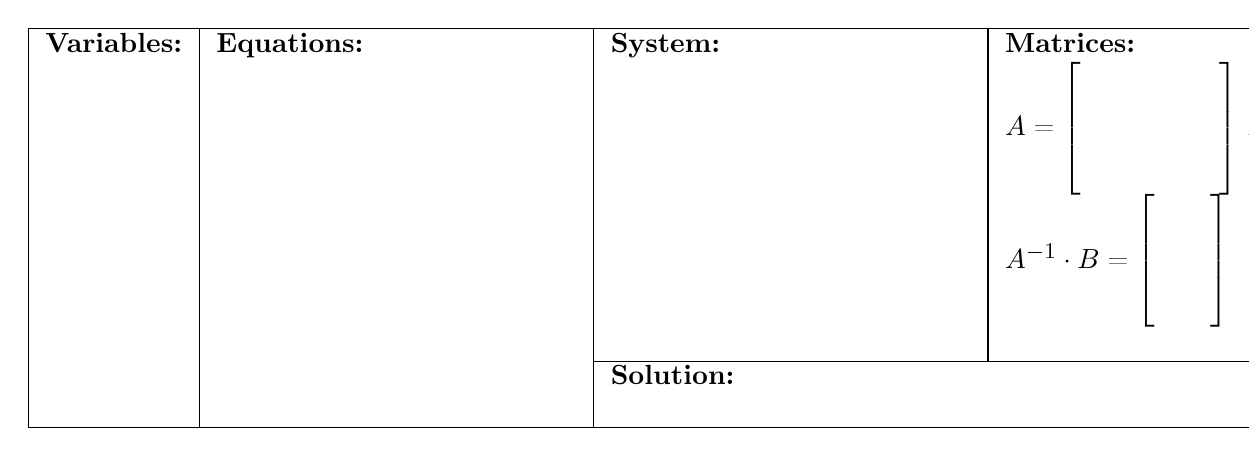
\begin{tikzpicture}
            \node
            [
                text width=1.25\textwidth, %I dinked with the multiplier to get balanced margins
                fill=white!30, 
                fill opacity=1,
                text opacity=1,
                inner sep=0pt,
            ]
            {%
                \begin{tabular}{|l|m{1.8in}|m{1.8in}|m{2.1in}|}
                    \hline
                    {\bfseries\scshape Variables:} & {\bfseries\scshape Equations:} & {\bfseries\scshape System:} & {\bfseries\scshape Matrices:} \\
                    % & & & \\
                    & & & 
                    \(
                        A = 
                        \begin{bmatrix}
                            \phantom{99} & \phantom{99} & \phantom{99} \\
                            \phantom{99} & \phantom{99} & \phantom{99} \\
                            \phantom{99} & \phantom{99} & \phantom{99} \\
                            \phantom{99} & \phantom{99} & \phantom{99} \\
                        \end{bmatrix}
                    \)
                    \(
                        B = 
                        \begin{bmatrix}
                            \phantom{999}\\
                            \phantom{999}\\
                            \phantom{999}\\
                            \phantom{999}\\
                    \end{bmatrix}
                    \)
                    \\
                    & & &
                    \(
                        A^{-1}\cdot B = 
                        \begin{bmatrix}
                            \phantom{9999}\\
                            \phantom{999}\\
                            \phantom{999}\\
                            \phantom{999}\\
                    \end{bmatrix}
                    \)
                    \\
                    & & & \\ \cline{3-4}
                    & & 
                    \multicolumn{2}{l|}{\bfseries\scshape Solution:}
                    \\ 
                    & & 
                    \multicolumn{2}{l|}{\,}
                    \\ 
                    \hline
                \end{tabular}
            };
        \end{tikzpicture}
    \end{adjustwidth}
}


{\small Pre-AP Algebra 2}\hfill Name: \rule{2in}{0.15mm}

{\Large PAP HW 4.4 (DAY 2) Matrix Applications}\hfill Period: \rule{0.5in}{0.15mm}

\begin{tcolorbox}
    \itshape\small
    These problems are {\bfseries\itshape almost} the same
    as the problems from yesterday. 
    The differences are that 
    \begin{itemize}[topsep=0in,itemsep=0em]
        \item I give you a {\bfseries\itshape different solution}.
        \item I ask you to change the problem so that it yields that different solution.
        \item Finally I want you to {\bfseries\itshape verify} 
        your answer by solving your changed problem and showing 
        that you got the different solution that I told you to start from.
    \end{itemize}
    \vspace{1em}
    You'll know you did it right if your solution in the last step
    gives you the different solution that I told you to start from.
    (So, sadly, I am not giving you the answers.)
\end{tcolorbox}




{\bfseries\large 1)} 
{\itshape
Rewrite problem (1) from yesterday's assignment so that 
the answer is 40 dimes and 60 quarters. (Fill in the blanks, and then verify 
that solving the problem gives you this answer.)
}

You find a jar of dimes and quarters.
There is a total of \gap{100} coins in the jar.
When you take them to the bank (to the coin counting machine),
you find that they added up to \gap{\$19.00}.
How many dimes and how many quarters were in the jar?

\myWideMatrixTable[-0.1in]

\vspace{0.5in}




{\bfseries\large 2)} 
{\itshape
Rewrite problem (2) from yesterday's assignment so that 
the answer is 500 pennies, 20 nickles, and 40 dimes. (Fill in the blanks, and then verify 
that solving the problem gives you this answer.)
}

You find another jar of \gap{560)} coins consisting of pennies, nickles and dimes.
You just happen to know that there are \gap{20} fewer nickles than dimes
(or equivalently, there are \gap{20} more dimes than nickles).
When you take them to the bank (to the coin counting machine),
you find that they added up to \gap{\$10.00}.
How many pennies, nickles, and dimes were in the jar?

\myWideMatrixTable[-0.1in]

\vspace{0.5in}


\newpage
{\bfseries\large 3)} 
{\itshape
Rewrite problem (3) from yesterday's assignment so that 
the answer is 500 carnations, 20 roses, and 40 daisies. (Fill in the blanks, and then verify 
that solving the problem gives you this answer.)
}

Jazmin's Restaurant ordered 2\gap{330} flowers for the holidays.
They ordered carnations, roses and daisies.
They ordered \gap{20} fewer roses than daisies
(or equivalently, \gap{20} more daisies than roses).
The carnations cost \$1.50 each.
The roses cost \$5.75 each.
The daisies cost \$2.60 each.
The total cost of the order was \gap{\$945.00}.
How many of each kind of flower did they order?

\myWideMatrixTable[-0.1in]

\vspace{0.5in}
\vfill





{\bfseries\large 5)} (Yes, I skipped problem 4.)
{\itshape
Rewrite problem (5) from yesterday's assignment so that 
the answer is 350 matinee tickets, 100 student tickets, and 200 regular tickets. 
Notice that the ``twice as many'' information is also different in this problem 
from the original problem 5.
(Fill in the blanks, and then verify 
that solving the problem gives you this answer.)
}

Last weekend, the Nostream Movie Theater sold a total of \gap{650} movie tickets.
They earned a total of \gap{\$4050.00}.
Tickets are sold in one of three ways:
\begin{itemize}[itemsep=0in]
    \item A matinee (early show) ticket costs \$5.00.
    \item A student all-day ticket costs \$6.00.
    \item Regular tickets cost \$8.50.
\end{itemize}
They sold twice as many {\bfseries\scshape regular} tickets as {\bfseries\scshape student} tickets.
How many of each kind of ticket did they sell?

\myWideMatrixTable[-0.1in]

\vspace{0.5in}
\hfill{\itshape (Ans: 900 matinee, 1800 student, 5800 regular)}
\vspace{2em}



\newpage
{\bfseries\large 6)} 
Make up a brand-new word problem like those from yesterday.
Make sure it involves {\bfseries\itshape three (3)} variables.
Do the following three things:
\begin{itemize}[itemsep=0in]
    \item Write your problem in words as if you were the teacher. 
    \item Give me the answers to your problem (the value of the three variables).
    \item And then show me how to correctly solve your problem as if you were a student.
\end{itemize}

Write your problem here:
\vfill

Write the correct answers to your problem here:
\vspace{1in}

Write the solution to your problem here:
\myWideMatrixTable[-0.1in]
\vspace{4em}

\end{document}